\documentclass[../main.tex]{subfiles}

\begin{document}
\chapter{What the hell is a vector?}

\section{What is a vector?}
Well, as the case with any definition we can always choose to make it whatever we want. :P
But in a less comical note many problems in the (real) world apparently can be represented and solved by using list of numbers as a fundamental tool.

Okay! So let's define \textbf{vector as just a list of numbers}. (Want to use the word sequence instead of list, but it might mean something else later on)

\section{For god sake, what is `dimensionality of vector' then?}
Well for example consider the following vectors

\begin{table}[h]
  \centering
  \begin{tabular}{ c  c  c }
    Vector name & Value & Dimension\\
    $ V_0 $ & () & 0\\
    $ V_1 $ & (1) & 1\\
    $ V_2 $ & ($\sqrt{2}$) & 1\\
    $ V_3 $ & (-100, $\sqrt{3}$) & 2\\
    $ V_4 $ & (0, 0.1) & 2\\
    $ V_5 $ & (0, 0, 0) & 3\\
    $ V_6 $ & (0, 1, 2, 3) & 4\\
  \end{tabular}
\caption{Dimensions of Vectors}
\label{tab:dim}
\end{table}

For each of the above vectors its dimensionality is written in the third column.
So for us the \textbf{dimension of a vector is just the count of numbers in the list}.
It is same as the length/size of the list. A vector with dimension N can be called ND-vector (spoken as N dimensional vector).

\pagebreak

\section{What is a co-ordinate system?}
Co-ordinate system is a method to represent the concept of `space' with real numbers.
A co-ordinate system consists of things called `axes'. The collection of `axes' is called the frame of co-ordinate system.
For any `point' in the `space' there is one and only one way of representation in reference to a frame, i.e. to give the signed lengths along each axis which one has to travel to from point which represents zero length in all axes (the origin) to get to the required point. The dimensionality of co-ordinate system is the number of axes of the co-ordinate system.

\begin{enumerate}
  \item Axis 1 + axis 2 + ... + axis N = co-ordinate frame
  \item Frame is used to reference to points
  \item Set of all points form a space
  \item Frame + space = system
  \item N = dimension of co-ordinate system
\end{enumerate}

\section{What is the deal with co-ordinate systems and vectors?}
We can think of \textbf{each number in vector as the signed length in each of the axes of an N dimensional co-ordinate frame}.
This way a numerical form of vector can be used to represent a point in space of appropriate dimension and a point can be used to visualize a numerical form of vector.

\begin{figure}[h]
  \centering
  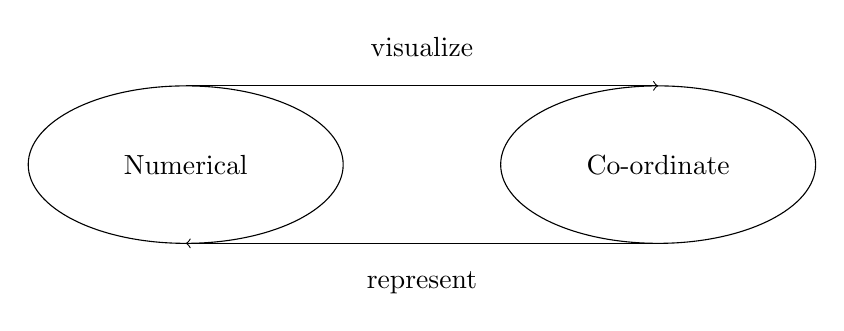
\begin{tikzpicture}
    \draw (-3, 0) ellipse (2cm and 1cm);
    \draw (-3, 0) node {Numerical};
    \draw (3, 0) ellipse (2cm and 1cm);
    \draw (3, 0) node {Co-ordinate};
    \draw[->] (-3, 1) -- (3, 1);
    \draw (0, 1.5) node {visualize};
    \draw[->] (3, -1) -- (-3, -1);
    \draw (0, -1.5) node { represent };
  \end{tikzpicture}
\end{figure}


For example a vector $ \blockcomment{Column-Vector: 2, -3} \begin{pmatrix} 2 \\  -3 \end{pmatrix} $  has dimensionality of 2, hence called a 2D vector and can be used to represent a point in a 2D co-ordinate space formed by 2D co-ordinate frame which consists of 2 axes. The point can be arrived at starting from the origin and moving 2 units along first axis and -3 units along second axis.

\begin{figure}[ht]
  \centering
  \begin{tikzpicture}
    \draw[step=1cm,gray,very thin] (-2.9,-3.9) grid (2.9,1.9);
    \draw[->] (-3, 0) -- (3, 0) node[anchor=north] {axis 1};
    \draw[->] (0, -4) -- (0, 2) node[anchor=east] {axis 2};
    \draw[thick, ->] (0, 0) -- (2, -3) node[anchor=west] { $ \blockcomment{Column-Vector: 2, -3} \begin{pmatrix} 2 \\  -3 \end{pmatrix} $  };
  \end{tikzpicture}
\end{figure}

Please note that
\begin{enumerate}
  \item There is no need to name these axes X and Y.
  \item There is no need for the axes to be perpendicular.
  \item No need for 1 unit along first axis to be same as 1 unit along second axis.
  \item No need for units of first axis to be same as the second one
\end{enumerate}

\section{Why like this?}
Well there is no specific reason. Just that it seems natural and seems to be useful to solve many problems in the world.

Probably the co-ordinate system was first developed to represent the objects in the real world with numbers. A co-ordinate system with dimensionality up to 3 makes sense in the real world. The ones with dimensionality 4 or above are not natural, as in we don't see physical manifestations of such systems. Umm... may be space time can be thought of as a 4D co-ordinate system with the 4th axis being time.

Anyway the most natural way to think about co-ordinate systems is to imagine a 3D co-ordinate system with axes placed spatially mutually perpendicularly and origin at the intersection of all of them.
\end{document}

